\documentclass[11pt]{article}
\usepackage[T1]{fontenc}
\usepackage[utf8]{inputenc}
\usepackage{tikz}
\usepackage{pgfplots}
\pgfplotsset{compat=1.18}

\title{TikZ and PGFPlots Validation}
\author{Validation Assets}
\date{}

\begin{document}
\maketitle

\section{Opaque graphics}
\label{sec:graphics}

Figure~\ref{fig:line} uses a tiny TikZ picture. Figure~\ref{fig:axis} uses a
minimal PGFPlots axis. Picture and axis bodies must stay opaque (CL-031,
CL-090, CL-091). Captions are translation candidates.

\begin{figure}[ht]
  \centering
  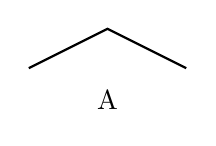
\begin{tikzpicture}
    \draw[thick] (0,0) -- (1,0.5) -- (2,0);
    \node at (1,-0.4) {A};
  \end{tikzpicture}
  \caption{Simple path diagram for opacity checks.}
  \label{fig:line}
\end{figure}

\begin{figure}[ht]
  \centering
  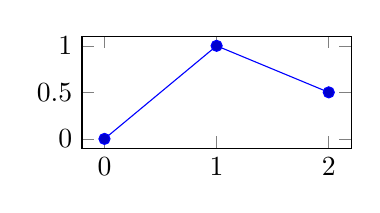
\begin{tikzpicture}
    \begin{axis}[
      width=5cm,
      height=3cm,
      xlabel={},
      ylabel={}
    ]
      \addplot coordinates {(0,0) (1,1) (2,0.5)};
    \end{axis}
  \end{tikzpicture}
  \caption{Minimal axis plot for PGFPlots opacity.}
  \label{fig:axis}
\end{figure}

Sync and fail-closed build must succeed with opaque regions intact (CL-092).

\end{document}
